\problemname{Delft Distance}

\newcommand{\maxw}{700}

\illustration{.25}{Watertoren}{Delft water tower. \\
	CC BY-SA 3.0 by Michiel1972 on \href{https://commons.wikimedia.org/wiki/File:Delft_-_Watertoren_(2010).jpg}{Wikipedia}}%
You are currently in your hotel at the north-west corner of Delft, and want to go to the contest site at the university in the south-east corner of Delft.
To get there, you have to go right through the historical centre of the city.
Like Manhattan, the city consists of a grid of $h \times w$ buildings.
But unlike Manhattan, the city does not only contain square residential buildings but also some round medieval towers.
All the square buildings are axis aligned with a side length of $10~\text{m}$ and all round towers have a diameter of $10~\text{m}$.
There is just enough space for a small alley of negligible width between two neighbouring buildings.

Since you are already late for the contest start, you need to find a shortest path from your hotel to the contest site.
Fortunately, you have a map of the city. See Figure~\ref{fig:d} for an example.

\begin{figure}[h]
	\centering
	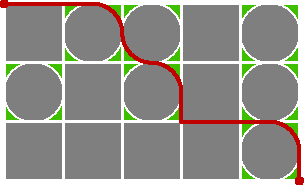
\includegraphics{sample}
        \caption{Illustration of Sample Input 1, with a shortest path shown in red.}
	\label{fig:d}
\end{figure}

\begin{Input}
	The input consists of:
	\begin{itemize}
		\item One line with two integers $h$ and $w$ ($1 \leq h,w \leq \maxw$), the number of rows and the number of columns of buildings shown on the map of the city.
		\item $h$ lines, each with $w$ characters which are either `\texttt{O}' (for round towers) or `\texttt{X}' (for square buildings) describing the shapes of the buildings.
	\end{itemize}
	The map is oriented with the north side up.
\end{Input}

\begin{Output}
	Output the length of a shortest path from the north-west corner to the south-east corner of Delft in metres.
	Your answer may have a relative or absolute error of at most $10^{-6}$.
\end{Output}
